\documentclass[handout]{beamer}

\usepackage[utf8x]{inputenc}
\usepackage{textcomp} 
\useoutertheme{lsp}

\usepackage{lsptitle}

\def\two@digits#1{\ifnum#1<10 0\fi\number#1}
\def\mytoday{\two@digits{\number\day}.\two@digits{\number\month}.\number\year}


\usepackage{xspace,multicol}
\newcommand{\latex}{\LaTeX\xspace}


\newcounter{lastpagemainpart}
\footnotesep0pt
\renewcommand{\footnoterule}{}
\usefootnotetemplate{
  \noindent
  \insertfootnotemark\insertfootnotetext}

\let\beamerfn=\footnote
\renewcommand{\footnote}[1]{%
\let\oldfnsize=\footnotesize%
\let\footnotesize=\tiny%
\beamerfn<\thebeamerpauses->{#1}%
\let\footnotesize=\oldfnsize}


\date{08.09.2014 Open-Access-Tage 2014 Köln}

\usepackage{eurosym} 
\usepackage{ogonek}  % Dabrowska
% \usepackage{libertine}

% Irgendein Font definiert mir das \dh wieder über.
\renewcommand{\centerline}[1]{\hfill#1\hfill\hfill\mbox{}}


\title{\mbox{Open-Access-Monographien}\\ in der Linguistik}
% \institute{FU Berlin}
\author[Nordhoff\&Siller]{Sebastian Nordhoff \& Debora Siller}



\begin{document}
\lspbeamertitle

\section{intro}
        Sprachwissenschaft
        DFG
        Geschichte
        stats
        Personal
            Front End
                Gamification
                Open Review
            Sys Admin
            R\&D
            Koordinator
            BWL
            
\section{Prinzipien}

\frame{
\frametitle{Prinzipien}
\begin{itemize}
 \item      Rückhalt
                Communitybuilding
                Jedes Buch muss in einer Reihe erscheinen
                    Reihenherausgeber organisieren selbständig       
 \item      Prestige
                soviel Prestige wie möglich in sowenig Zeit wie möglich
                Champions League      
 \item      betriebswirtschaftliche Fundiertheit       
\end{itemize}

        Platinum OA
        
}

\section{Stand}

\frame{
\frametitle{Stand}
teaser
}

\frame{
\frametitle{Prestige: Satz und Druck}
\begin{itemize}
\item 
\end{itemize}
}

\frame{
\frametitle{Prestige: Satz und Druck}
\begin{itemize}
\item                 Satz und Druck
                    Glyphen
                        echtes Unicode
                        Erweiterung der Fonts
                    Chinesisch, Hebräisch, Arabisch
                    diverse fachspezifische Erweiterungen
                    Ligaturen
                    Indexe
                    Querverweise
                    PoD

\end{itemize}
}

\frame{
\frametitle{Inhalt}
\begin{itemize}
\item     Peer review
                    keine Dissertationen
                soziale Qualität
                    priominente Unterstützer
\end{itemize}
}

\frame{
\frametitle{Statistik}
\begin{itemize}
\item Reihen:
  \begin{itemize}
   \item        projiziert: 2014: 5 2015:7 2016:9
    \item            Bei Start 9
    \item           Jetzt 13, Ende des Monats wahrscheinlich 14         
  \end{itemize}
\item Bücher:
   \begin{itemize}
    \item       39 Anfragen
    \item                    14 akzeptiert (in 6 Reihen)
 \item                       2 veröffentlicht
                 \item       6 abgelehnt        
   \end{itemize}
\end{itemize}
}

\frame{
\frametitle{Rückhalt: Mobilisierung}
\begin{itemize}
\item 
                Supporterseite
                Mailingliste
                Pledge to Publish
                kritische Masse
                Start auf der DGfS mit dem ersten Buch 7 Tage nach Projektbeginn
\end{itemize}
}

\frame{
\frametitle{Rückhalt: Einbindung}
\begin{itemize}
\item     Unterstützer: 479
\item     reader 286
\item     reviewer 276
\item     series editor 24
\item     Proofreader: 80 (15)
\item     Setzer: 32(6)
\item Font Designer
\item Grafik-Designer
\item Latex-Entwickler      
\end{itemize}
}

\frame{
\frametitle{BWL}
\begin{itemize}
\item       Zusammenarbeit mit dem Lehrstuhl für Wirtschaftsinformatik der FU
\item       Studentischer Businessplan liegt vor, wird in Teilen in eigentlichen Businessplan übernommen
\item       proaktive Gestaltung der Dienstleistungslandschaft
    \begin{itemize}
    \item    PoD-Service
    \item    Konversionsdienstleister doc2tex
    \end{itemize}
\end{itemize}
}

\frame{
\frametitle{Kostenplan}
\begin{itemize}
\item Personal,  Sachmittel, Reise, PR, Infrastruktur
\end{itemize}
}


\frame{
\frametitle{Modelle für die Zukunft}
% 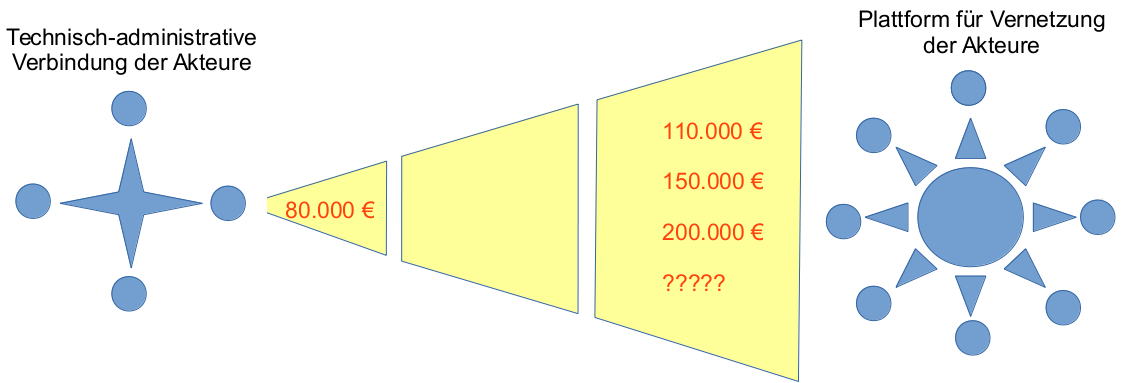
\includegraphics{modelle.png}
}

\frame{
\frametitle{Finanzierung für die Zukunft}
% 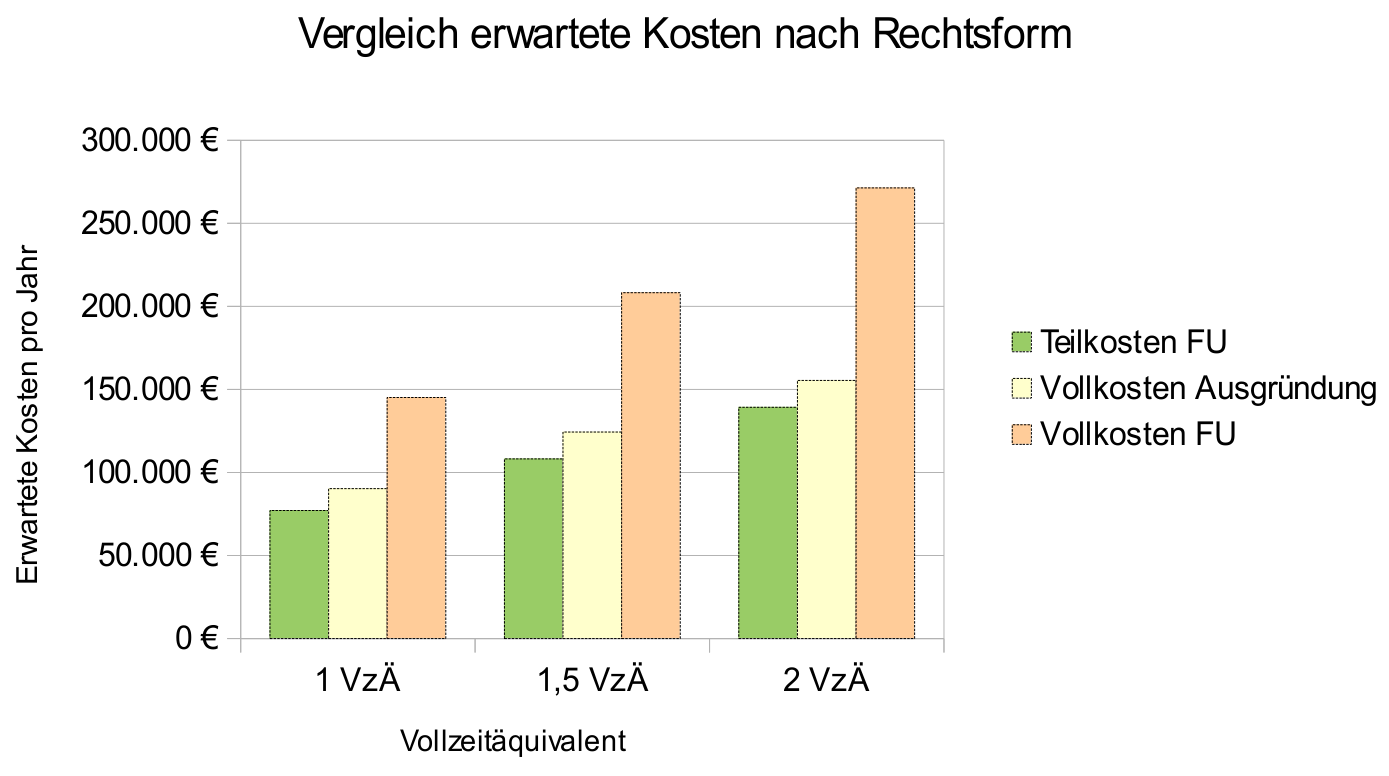
\includegraphics{finanzierung.png}
}


\end{document}


                
                
                
                
        VWL
            Geldquellen
                letztendlich immer öffentliche Hand
                Formen
                    Reader-pays
                    Author-pays
                    Government pays
                    Learned Society pays
                        Beispiel Med
                    community pays
                Fallen
                    Reader-pays
                        bekannt
                    Author-pays
                        Preissteigerung durch Prestige
                    Government pays
                        kein Wettbewerb
                    Learned Society pays
                    community pays
                        Unischerheit
                Fördermodell
            Interessenlagen
                Regierung
                    wenig Geld ausgeben
                    viel Forschung
                    Volksbildung
                Autoren
                    wenig Geld ausgeben
                    viele Prestige
                    viele Zitationen
                    wenig Aufwand
                Leser
                    wenig Geld ausgeben
                    Qualität
                    freier Zugang
                Learned Society
                    freie Veröffentlichung
                    freier Zugang
                    Qualität
                Bibliotheken


\end{document}


\section{Hintergrund}
 
\frame{
\frametitle{Hintergrund}

\begin{itemize}[<+->]
\item 06.2012 Treffen mit Adele Goldberg, Thomas Herbst, Anatol Stefanowitsch
\item 08.2012 OALI-Webseite, Mails an prominente Kollegen
\item 08.2012 Treffen mit Martin Haspelmath
\item 10.2012 Kick-Off-Treffen an der FU-Berlin mit internationaler Beteiligung via Skype (Anke
  Lüdeling, Gereon Müller, FU-Linguistik, \ldots)
\item 02.2013 Einreichung Antrag im DFG-Programm \emph{Wissenschaftliche Monographien und monographische Serien im Open Access}
\item 12.2013 DFG-Finanzierungszusage, 2 von 17 Projekten gefördert, $>$~575,000 € für zwei Jahre,
  72\,\% der Gesamtfördersumme
\item 02.2014 Einstellung Koordinator
\item 03.2014 Publikation der ersten Bücher
\item 09.2014 39 Anfragen, 14 angenommene Bücher, 2 veröffentlichte Bücher

\end{itemize}

} 

\frame{
\frametitle{Gemeinschaftsprojekt}

\begin{itemize}[<+->]
\item 426 Unterstützer, über 100 sehr prominent, viele anwesend

siehe: \url{http://langsci-press.org/Meta/sign/supporters}

\item Unterschreibe auch du!

\url{http://langsci-press.org/Meta/sign/}

\item dezentrale Organisation

\begin{itemize}
\item nur Bücher in Reihen
\item Reihenherausgeber übernehmen Verantwortung und steuern Ressourcen bei
\item Reihenvorschläge werden vom Advisory Board evaluiert
\item Satz, Korrekturlesen durch Herausgeber bzw.\ die Community
\end{itemize}

\item Speicherung, Archivierung und Katalogisierung durch FU-Bibliothek

\item Print on Demand mit verschiedenen Anbietern und Vertrieb über bekannte Kanäle
\end{itemize}
}


\frame{
\frametitle{Reihen}

\begin{itemize}[<+->]
\item African Language Grammars and Dictionaries
\item Comparative Studies on Niger-Congo Languages
\item Studies in Diversity Linguistics
\item Empirically Oriented Theoretical Morphology and Syntax
\item Implemented Grammars
\item Lecture Notes in Language Sciences
\item Studies in Laboratory Phonology
\item Topics at the Grammar-Discourse Interfaces\\
\item Translation and Multilingual Natural Language Processing\\
\item Computational Models of Language Evolution
\item Conceptual Foundations of Language Science
\item Language Variation
\item Studies in Caribbean Languages
\end{itemize}
}

\section{Statistik}

\frame{
\frametitle{Statistik}

\begin{itemize}[<+->]
\item In Vorbereitung: 19 
\item Eingereicht: 13 
\item Angenommen: 14 
\item Abgelehnt: 6
\end{itemize}

}

\frame[shrink=15]{
\frametitle{Projektbestandteile}

\begin{itemize}[<+->]
\item Schaffung von Standards für \latex-Templates in der Linguistik
\item Automatische Konversion von \latex in diverse andere Formate\\
      (XML, e-books)
\item Schaffung einer Literaturdatenbank für Linguistik und Aufnahme entsprechender Einträge in \url{http://glottolog.org/}
\item Enhanced Publication
      \begin{itemize}
      \item ausklappbare Syntaxbäume (\url{http://hpsg.fu-berlin.de/OALI/rec2/rec2.html})
      \item Speicherung von Korpusdaten
      \item Sound-Dateien
      \item \ldots
      \end{itemize}
\item Erweiterungen von Open Monograph Press
      \begin{itemize}
      \item Anpassung an die deutschen Besonderheiten (VG-Wort, Kataloge, \ldots)
      \item Open Review (optional)\nocite{Pullum84a}
      \item Diskussionsphasen vor endgültiger Veröffentlichung (optional)
      \item Gamification (optional)
      \end{itemize}
\item alle Ergebnisse Open Source und für andere Disziplinen/Projekte zur Nachnutzung
\end{itemize}

\nocite{MH2013a}

}

\frame{
\frametitle{Stellen}
\begin{itemize}[<+->]
\item 1 Stelle: \latex/XML
\item 1 Stelle: Open Monograph Press-Erweiterungen
\item 1/2 Stelle: Support/Betreuung von Herausgebern/Autoren am CeDiS
\item 1/2 Stelle: BWLer: Dokumentation der Kosten, Geschäftsmodell\\
      (optionales Author Pays, optionale Bibliotheksbeiträge, Micropayment-Spenden, \ldots)
\bigskip
\item Ausschreibung in den nächsten Tagen
\end{itemize}
}

\section{Ausblick}

\frame{
\frametitle{Wie geht's weiter?}

\begin{itemize}
\item Farbe bekennen: \url{http://langsci-press.org/Meta/sign/}

(unser kleines \url{thecostofknowledge.com})

\item Mit anderen reden

\item Buch schreiben

\item Sich darüber freuen,\\ 
      dass das Buch auf der ganzen Welt gelesen werden kann.

\end{itemize}

}
\nocite{Shieber2012a}
\makeatletter
\setcounter{lastpagemainpart}{\the\c@framenumber}
\makeatother


\appendix

\section{Preise}

\frame{
\frametitle{Preisliste für \\Open-Access-Bücher}

\begin{itemize}
\item Palgrave Macmillan: 11,000 £ (17,500 \$)\footnote{
\url{http://poynder.blogspot.co.uk/2013/09/de-gruyters-sven-fund-on-state-of-open.html}. 04.03.2014.
}
\item Springer: ca.\, 15,000 €\footnote{
\url{http://poynder.blogspot.co.uk/2013/09/de-gruyters-sven-fund-on-state-of-open.html}. 04.03.2014.
\newline
Lustigerweise steht das nicht in der FAQ: \url{http://www.springeropen.com/about/faq/chargesbooks}. 04.03.2014.
}
\item De Gruyter Open: 10.000 € (p.\,M.\ 02/2014)\\
      (1.500€ bei normalen Büchern, wenn nicht selbst gesetzt)
\item Brill: 5.000 €
\item Language Science Press: 0 €\\
      (Spenden und Publikationsmittel aus Projektgeldern willkommen)
\end{itemize}

}

\mode<beamer>{

\setcounter{framenumber}{\thelastpagemainpart}



\end{document}